\chapter{Použitie viacerých template štruktúr pri predikcii}

Ako druhé opatrenie, na zlepšenie rýchlosti a presnosti predikovania nekonzervovaných úsekov sme navrhli  použiť viacero template štruktúr na predikciu jednej target štruktúry tak, že ich použijeme spolu na vytvorenie jednej štruktúry konzervovaných úsekov. Očakávali sme pritom, že sa nám podarí zmenšiť počet a dĺžku nekonzervovaných úsekov v predikovanej štruktúre a tým výrazne zjednosušiť ich predikciu algoritmom FARFAR.

\section{Výber sekundárnych template štruktúr}
Hlavnou myšlienkou algoritmu je použiť viacero template štruktúr pre predikciu jednej target štruktúry. Tým môžeme dosiahnuť väčšiu percentuálnu mieru konzervovaných úsekov v štruktúre, čo by malo zjednodušiť následnu predikciu nekonzervovaných úsekov.


\indent  Existuje viacero spôsobov, ktorými je možné predikovať target molekulu pomocou viacerých template molekúl. Jeden prístup by mohol byť rozdeliť si target sekvenciu na regióny a pre predikciu každého regiónu použiť inú template štruktúru. My sme sa aj vzhľadom na jednoduchšiu implementáciu do už existujúceho algoritmu rozhodli postupovať tak, že používame jednu template štruktúru ako primárnu (hlavnú) a ďalšie template štruktúry, ako sekundárne (vedľajšie), ktoré sú použité na vyplnenie dlhých nekonzervovaných úsekov (to sú tie, ktoré v pôvodnom algoritme vyčleňujeme do samostatných predikcií v metóde \textit{ProcessLongUnconservedParts}).    


\indent Potencionálne spôsoby ako nájsť vhodné sekundárne template štruktúry pre nekonzervované úseky sú: 
\begin{enumerate}
\item Globálne zarovnanie potenciálnych sekundárnych temeplate molekúl s target molekulou. 
\item Lokálne zarovnanie potenciálnych sekundárnych template molekúl s target molekulou. 
\item Semiglobálne zarovnanie potenciálnych sekundárnych temeplate molekúl s target molekulou. 
\item Najprv zarovnať heuristickým algoritmom (BLAST, FASTA) \cite{BLAST} a následne z takto vybranej skupiny najlepších štruktúr vybrať tú najvhodnejšiu za pomoci jedného z troch hore uvedených spôsobov.
\end{enumerate}


\indent My sme najprv skúšali prvý a najjednoduchší postup, a to globálne zarovnávať potencionálne sekundárne template molekuly na target molekulu, pričom hľadáme takú sekundárnu template štruktúru, ktorá by dobre vyplnila nekonzervované úseky (teda by ich pokryla aspoň na 60\%, ktoré sme na základe doterajšieho testovania určili ako dolnú hranicu pokrytia v zarovnaní). Pri globálnom zarovnaní sme však nenachádzali vhodné sekundárne template štruktúry, ktoré by pokrývali nekonzervované úseky s aspoň 60\%. Je to dané tým, že okrem toho, že v sekundárnej template štruktúre sa musí nachádzať vhodný konzervovaný úsek, musí byť aj na správnom mieste v sekvencii tak, aby bol globálne zarovnaný na miesto nekonzervovaného úseku v target sekvencii. Tento prístup sme nakoniec označili za nepoužiteľný.


\indent Lokálne zarovnanie hľadá zarovnanie s najlepším skóre dvoch podúsekov z target aj template sekvencie. To znamená, že dĺžka zarovnaných úsekov je určená najvyšším skóre zarovnania oboch sekvencií (ak by bol do zarovnania pridaný alebo odobratý ľubovolný nukleotid z target alebo template sekvencie skóre zarovnania by sa zhoršilo). Vzhľadom na to, že my potrebujeme zarovnať celý nekonzervovaný úsek target sekvencie na ľubovoľný úsek template sevencie bolo by lokálne zarovnanie ťažko použiteľné.


\indent Semiglobálne zarovnanie je kombinácia globálneho a lokálneho zarovnania. Funguje tak, že kratšiu štruktúru zarovná na časť dlhšej štruktúry a nezarovnané úseky pred a po kratšej štruktúre sa do výsledného skóre zarovnania nezapočítavajú. Teda z globálnym zarovnaním má spoločné to, že kratšia sekvencia je zarovnaná celá na časť dlhšej. Z lokálnym zarovnaním má spoločné to, že pridaním alebo odobratím ďalšieho nukleotidu z dlhšej štruktúry do zarovnania by sme výsledné skóre len zhoršili. V našom algoritme ho budeme používať na vyľadanie optimálnych sekundárnych template molekúl. Postupovať budeme tak, že vyberieme nekonzervovaný úsek z target sekvencie a postupne ho budeme zarovnávať na rôzne potencionálne template sekvencie. Buď môžeme prejsť všetky dostupné sekvencie pre každý nekonzervovaný úsek a vybrať najlepšiu, alebo vyberieme prvú ktorá splní nejaké nami zadané požiadavky. My sme zvolili spôsob, kedy vyberieme prvú vhodnú template štruktúru, ktorú nájdeme.


\indent Semiglobálne zarovnanie získavame rovnakým nástrojom ako globálne, teda pomocou programu Emboss.Needle \cite{Emboss}. Z výsledného zarovnania nás nezaujíma skóre zarovnania, ale percentuálny pomer správne zarovnaných nukleotidov oproti nesprávne zarovnaným nukleotidom, prípadne medzerám v  zarovnaní (bez medzery na začiatku a na konci), čo označujeme ako podobnosť, alebo tiež similarity. Emboss ale do výstupného súboru zarovnania uvádza len globálnu podobnosť v kombinácií so semiglobálnym skóre \autoref{obr06:emboss}. To pre nás znamenalo, že sme museli naimplementovať parser, ktorý je založený na regulárnych výrazoch, vyberie zo zarovnania len zarovnanú časť a na základe toho určí percentuálnu podobnosť zarovnania.
\begin{figure}%[p]\centering
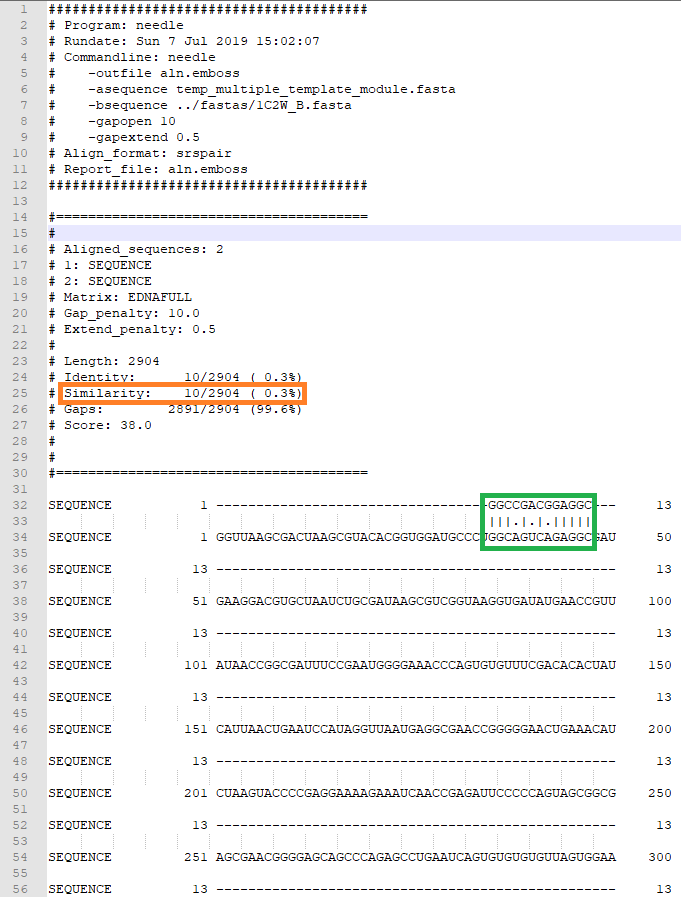
\includegraphics[width=\textwidth]{../img/emboss}
\caption{Príklad semiglobálneho zarovnania nekonzervovaného rozšíreného úseku dlhého 13 nukleotidov na sekvenciu 1C2W\_B dlhú 2904 nukleotidov. Zeleným obdĺžnikom je ohraničené zarovnanie, ktorého podobnosť nás zaujíma a oranžovým obdĺžnikom je označená hodnota globálnej podobnosti vypočítanej programom Emboss.}
\label{obr06:emboss}
\end{figure}


\section{Algoritmus}
\indent Kroky algoritmu používajúceho viacero sekundárnych template štruktúr:
\begin{enumerate}
\item Nájdeme dlhé nekonzervované úseky \textit{IdentifyLongUnconservedRegions}.
\item Otagujeme a vyfiltrujeme potenciálne template štruktúry sekvenčným prechodom všetkých štruktúr, uložíme  ich do poľa \textit{FindPotentialTemplates}.
\item Pre každý nekonzervovaný úsek:
\begin{enumerate}
\item Upravíme nekonzervovaný úsek na rozšírený nekonzervovaný úsek (o úseky, ktorými budeme spájať s primárnou target štruktúrou) \textit{ExtendGap}.
\item Pomocou semiglobálneho zarovnania nájdeme v indexovaných štruktúrach vhodnú sekundárnu štruktúru pre nekonzervovaný úsek \textit{FindTemplateForGap}.
\item Namapujeme vybraný fragment sekundárnej target štruktúry na príslušné miesto v template štruktúre (preindexovanie nukleotidov v sekundárnej template štruktúre) \textit{MapTemplateToGap}.
\item Vykonáme jeden z následujúcich dvoch krokov, podľa verzie algoritmu \textit{IntegrateNewTemplateStr}:
\begin{enumerate}
\item Dáme do superpozície štruktúru tvorenú konzervovanými úsekmi z primárnej template štruktúry a fragment zo sekundárnej template štruktúry.
\item Uložíme fragment sekundárnej template štruktúry do separátneho súboru, ktorý potom poskytneme algoritmu FARFAR.
\end{enumerate}
\end{enumerate}
\end{enumerate}


\indent Logika algoritmu je naimplementovaná v metóde \textit{MultipleTemplateModule}. Superimposer použitý v metóde \textit{IntegrateNewTemplateStr} bol pôvodne inšpirovaný skriptom od Anders S. Christensen-a dostupného na \url{https://gist.github.com/andersx/6354971} a výrazne upravený.  


\indent V prvom kroku sekvenčne prejdeme target štruktúru skladajúcu sa zatiaľ len z konzervovaných úsekov primárnej template štruktúry a vyhľadáme nekonzervované úseky dlhšie ako určitá hranica daná parametrom (momentálne nastavené na 7 nukleotirdov).


\indent V druhom kroku si predpripravíme potenciálne template štruktúry tak, že odstránime tie, ktoré obsahujú viac ako 5\% neplatných nukleotidov (znaky iné ako A,C,G,U). Okrem toho si uložíme dĺžku každej sekvencie a v nasledujúcom kroku budeme na seba zarovnávať len dosť dlhé sekvencie vzhľadom k nekonzervovanému úseku (minimálne 0,8 násobok dĺžky úseku). Dôvody sú vyhnutie sa problémovým dátam a ušetrenie času pri zarovnávaní hlavne dlhších nekonzervovaných úsekov. Bolo by možné si potenciálne template sekvencie predpripraviť mimo algoritmu predikcie, potom by ale bolo treba takto pripravené dáta prepočítavať pri zmene v databázi. Vzhľadom na to, že celý tento proces trvá pár sekúnd rozhodli sme sa robiť to vždy odznova počas predikcie.


\indent V ďalších krokoch iterujeme cez všetky vybrané nekonzervované úseky sekvencie a pre každý aplikujeme rovnaké kroky. Najprv si nekonzervovvaný úsek rozšírime. To znamená, že k nemu pridáme z oboch strán určitý počet nukleotidov (my používame parameter 5). Keďže pracujeme s nekonzervovaným úsekom musí existovať na každej strane minimálne 1 nukleotid, ktorý tento úsek ohraničuje (s výnimkou začiatku a konca sekvencie). Za pomoci týchto rozširujúcich nukleotidov sme schopní superpoziciovať (správne umiestniť) v nasledujúcich krokoch vybraný fragment sekundárnej template štruktúry do primárnej template štruktúry.


\indent V  kroku 3b postupne zarovnávame rošírený nekonzervovaný úsek s vyhovujúcimi predpripravenými štruktúrami z druhého kroku. V prípade, že zarovnanie splňuje určené podmienky, vyberieme príslušnu štruktúru za sekundárny template  pre spracovávaný nekonzervovaný úsek a v prehľadávaní ďalej nepokračujeme. Podmienky pre výber používame nasledujúce: podobnosť zarovnania minimálne 70\% a maximálne 95\%. Maximálnu podobnosť volíme preto, aby sme ako template nepoužili štruktúru skoro úplne zhodnú s target štruktúrou. To by síce bolo žiaduce pri naozajstnej predikcii, kedy chcem dostať čo najlepší výsledok, ale nežiadúce pre testovanie funkčnosti predikcie, kedy by nám to zvyšok predikcie výrazne zjednodušilo. Pri predikcií neznámej štruktúry tiež typicky nepoznáme žiadnu veľmi podobnú štruktúru neznámej štruktúre, inak by sme ju použili ako primárny template. 


\indent V ďalšom kroku musíme namapovať nukleotidy zo sekundárnej template štruktúry do nekonzervovaného úseku primárnej template štruktúry (ktorá je už namapovaná na target sekvenciu) podľa zarovnania. To znamená pre každý použitý nukleoti zistiť, na aký nukleotid bol v zarovnaní namapovaný a zmeniť jeho index v pdb súbore. Okrem toho musíme zmeniť aj chain ID v prípade, že sa nezhodujú chain ids primárnej a sekundárnej template štruktúry.


\indent V poslednom kroku sme skúšali dva rôzne prístupy. 
\begin{enumerate}
\item Superpoziciovanie sekundárnych template štruktúr do dlhých nekonzervovaných úsekov primárnej template štruktúry.
\item Uložiť fragmenty vypĺňajúce dlhé nekonzervované úseky do separátnych súborov.
\end{enumerate}

\indent Prvý spôsob je superpoziciovanie nukleotidov, ktorými sme rozšírili z oboch strán nekonzervovaný úsek a našli preň vhodnú sekundárnu template štruktúru.Tieto dodatočne pridané nukleotidy superpoziciujeme na odpovedajúce nukleotidy v primárnej template štruktúre. Inak povedané to znamená vhodným spôsobom rotovať a posúvať sekundárnu template štruktúru ako celok tak, aby sme minimalizovali RMSD nukleotidov, ktoré sa nachádzajú v oboch štruktúrach a majú rovnaké indexy. Na toto sme použili \textit{Superimposer} implementovaný v knižnici \textit{BioPython} \textit{https://biopython.org/}. Po vhodnej rotácií a translácií terciárnej template štruktúry z nej odstránime pridané rozširujúce úseky (pridané v metóde \textit{ExtendGap}) a nukleotidy čiastočne pokrývajúce nekonzervovaný úsek skopírujeme do primárnej template štruktúry. Takýmto spôsobom v ideálnom prípade vyplníme jeden dlhý nekonzervovaný úsek v primárnej template štruktúre, fragmentom štruktúry zo sekundárnej target štruktúry. Vo výsledku by sme pri použití tohoto prístupu mali template štruktúru, ktorá má dodatočne doplnené dlhé nekonzervované úseky vhodnými fragmentmi ostatných štruktúr. 


\indent Druhý prístup je jednoduchší a pozostáva len z uloženia správne namapovaných fragmentov sekundárnej template štruktúry do separátneho pdb súboru. Vo výsledku by sme teda mali pdb súbor s primárnou template štruktúrou a pre každý dlhý nekonzervovaný úsek v tejto štruktúre, by sme mali pdb súbor s fragmentom so sekundárnej template štruktúry vypĺňajúcej tento nekonzervovaný úsek. Fragmenty sukundárnych template štruktúr obsahujú informáciu iba o  relatívnej polohe nukleotidov v jednom fragmente a poloha štruktúr v rôznych nekonzervovaných úsekov je nezávislá.


\indent Posledná zmena, platná pri oboch dvoch prístupoch je, že vzhľadom nato, že sme našli sekundárne template štruktúry pre nekonzervované úseky nebudeme používať metódu \textit{ProcessLongUnconservedParts} z pôvodného algoritmu, ktorá vyčleňovala predikciu dlhých nekonzervovaných úsekov do samostatnej predikcie algoritmom FARFAR.


\indent Pre lepšie vysvetlenie uvádzame pseudokód algoritmu používajúceho viacero template štruktúr spolu s integráciou do pôvodného algoritmu. Pseudokód vychádza z pseudokódu algoritmu Trooper so sekundárnou štruktúrou predstaveného v piatej kapitole \autoref{kap5:pseudocode}.
\lstset{numbers=left, numberstyle=\tiny, stepnumber=1, numbersep=5pt}
\begin{lstlisting}
Main(fastaTarget, fastaTemplate
        , secStrTemplate, pdbTemplate)
{
   CheckTemplateMapping
      (fastaTemplate,pdbTemplate)
   alignment := Align
      (fastaTarget, fastaTemplate)
   alignment1 := UseSlidingWindow
      (alignment)
   alignment2 := ProcessGaps
      (alignment1)
   conservedParts := CopyConservedParts
      (alignment2, pdbTemplate)
   mappedConservedParts := MapConservedParts
      (conservedParts, alignment2)
   conservedPartsSecStr := CopyConservedPartsSecStr
      (alignment2, secStrTemplate)
   mappedConservedPartsSecStr := MapConservedPartsSecStr
      (conservedPartsSecStr, alignment2)
   predictedSecStr := PredictUnconservedSecStr
      (mappedConservedPartsSecStr)
   mappedConservedParts := MultipleTemplatesModule
      (mappedConservedParts)
   longParts[] := ProcessLongUnconservedParts
      (mappedConservedParts, secStr)
   shortParts[] := ProcessShortUnconservedParts
      (mappedConservedParts, secStr)
   predictedParts[] := PredictUnconservedParts
      (longParts[], shortParts[])
   finalModel := ConnectPredictedParts
      (predictedParts)
}

MultipleTemplatesModule(mappedConservedParts)
{
   gaps[] := IdentifyLongUnconservedRegions
      (mappedConservedParts)
   potentialTemplateStructures[] = FindPotentialTemplates
      (database)
   foreach gap in gaps
   {
      extendedGap = ExtendGap(5 nk from each side)
      secTemplate := FindTemplateForGap
         (extendedGap, potentialTemplateStructures) 
      preparedSecTemplate := MapTemplateToGap
         (secTemplate)
      mappedConservedParts := IntegrateNewTemplateStr
         (prepared_sec_template)
   }
   return mappedConservedParts
}

   FindTemplateForGap(gap, potentialTemplateStructures) 
   {
       alns = []
       foreach sequence in potentialTemplateStructures:
       {
          alns = EmbossAlign(sequence, gap)
       }
       bestAln = alns.SelectBest()
       return bestAln
   }

   MapTemplateToGap(secTemplate)
   {
      from secTemplate select only relevant nukleotides
      renumber secTemplate to match unconserved region
      rename chain to match the primary template
   }   

   IntegrateNewTemplateStr(preparedSecTemplate)
   {
      superimpose prepared template to gap
      OR
      save secondary template to new file
   }

\end{lstlisting}

\section{Integrácia do existujúceho algoritmu}
Integácia do algoritmu si vyžiadala niekoľko úprav v pôvodnom algoritme a implementácií.

\indent Kostra algoritmu, používajúceho viacero template štruktúr:
\begin{enumerate}
\item Vybrať primárnu target štruktúru.
\item Zarovnať  target a template sekvencie pomocou algoritmu globálneho zarovnania.
\item Identifikovať dlhé nekonzervované úseky v zarovnaní.
\item Pre každý nekonzervovaný úsek nájsť vhodnú sekundárnu target štruktúru pomocou semiglobálneho zarovnania.
\item Integrovať príslušné fragmenty zo sekundárnych template štruktúr do konzervovaných úsekoch z template štruktúry (pomocou superpozície), alebo fragmenty uložiť do separátnych súborov.
\item V prípade vyplnenia nekonzervovaného úseku sekundárnou template štruktúrou nemusíme vyčleňovať extra predikcie pre dlhé nekonzervované úseky.
\item Upravíme vstupy pre FARFAR
\item Pokračujeme predikciou algoritmom FARFAR.
\end{enumerate}


\indent Prvé tri kroky sa v ničom nelíšia od pôvodného algoritmu. Najprv musíme získať hlavnú template štruktúru, pričom nezáleží na tom, či ju už dostaneme na vstupe, alebo ju budeme algoritmicky hľadať  nejakú vhodnú v našej stiahnutej databáze štrutúr. Následne zarovnáme target a template sekvencie, aplikujeme algoritmus posuvného okienka, ošetríme medzery v zarovnaní a dostaneme tak nekonzervované úseky, ktoré musíme predikovať. Z nich vyberieme tie dlhé a pokúsime sa pre ne nájsť sekundárne template štruktúry. Ktoré použijeme podľa popisu algoritmu uvedeného v predchádzajúcej sekcií.


\indent V nasledujúcich krokoch nepoužijeme metódu \textit{ProcessLongUnconservedParts}, ktorá vyberá a separátne pripravovuje predikciu dlhých nekonzervovaných úsekov, pretože tieto by mali byť doplnené zo sekundárnych template štruktúr a preto táto metóda stráca význam. Okrem toho musíme upraviť vstupné súbory a volania algoritmu FARFAR o novo pridané nukleotidy a súbory. Následne v prípade, že používame druhú variantu algoritmu s viacerými template súbormi, musíme upraviť automatizačné shell scripty, aby tieto súbory nakopírovali na správne miesto spolu s ostatnými vstupnými súborm algortimu FARFAR.


\section{Časová zložitosť} 
V tejto sekcií popíšeme, ako sa líši časová zložitosť od pôvodného algoritmu Trooper. Jediná zásadná funkcionalita, ktorá pribudla, je implementovaná v metóde \textit{MultipleTemplatesModule}.
Z pohľadu asymptotickej zložitosti je zaujímavá hlavne metóda  \textit{FindTemplateForGap} slúžiaca na vyhľadanie sekundárnych template štruktúr. Metóda zarovnáva nekonzervovaný úsek na každú sekvenciu v databáze. Z toho vychádza časová zložitosť \textit{O(ng$l^2$)}, pričom \textit{n} je počet štruktúr v databáze, \textit{g} je počet nekonzervovaných úsekov (ich počet však bude funkčne závislý od dĺžky target štruktúry - čím dlhšia, tým viac nekonzervovaných úsekov)  a \textit{l} je dĺžka štruktúry v databázi. Vo výsledku sa nám teda asymptotická časová zložitosť zhoršila z \textit{O($l^2$)} na \textit{O(ng$l^2$)}.


\indent Reálna dĺžka behu algoritmu výrazne narástla. Merali sme ju na počítači s procesorom Intel Core i5-6200Li 2,8GHz a jeden beh metódy \textit{FindTemplateForGap} trval pri nekonzervovanom úseku dĺžky 7-25 nukleotidov približne 30 sekúnd, pričom sme ale gap zarovnávali na celú databázu štruktúr a nie len tie dĺžky 50-500 nukleotidov. Celková dĺžka behu je potom závislá na počete dlhých nekonzervovaných úsekov, ktoré predikovaná štruktúra obsahuje (pre štruktúry dĺžky 50-500 nukleotidov a podobnosti s primárnym template-om 60-90\% sú to  najčastejšie 0 až 3 úseky). 


\indent Zvýšená časová náročnosť by sa možno dala riešiť použitím algoritmov FASTA alebo BLAST, ktoré používajú heuristické metódy na vyhľadanie najpodobnejších sekvencií. Vzhľadom na to, že predikcia predikcia algoritmom FARFAR trvá oveľa dlhšie, rozhodli sme sa tento problém neriešiť.


\section{Experiment a výsledky} 
Pre experiment sme volili rovnaké podmienky a vstupné parametre, ako pre predchádzajúce dva experimenty. Predikovali sme tiež s použitím sekundárnej štruktúry, pretože predikcia so sekundárnou štruktúrou, ako aj predikcia s viacerými template štruktúrami sú navzájom kompatibilné. Experimnety sme vykonávali na oboch variantách metódy \textit{IntegrateNewTemplateStr}.


\indent Prvý spôsob predikcie vypĺňaním nekonzervovaných úsekov v primárnej template štruktúre sa nám nepodarilo dokončiť, pretože sme naše zásahy do štruktúry nedokázali zladiť s algoritmom FARFAR. Vzhľadom na to, že pre nás funguje ako čierna skrinka, a neexistuje podrobná dokumentácia, ktorá by vysvetľovala príčiny chýb, ktoré môžu nastať sme s týmto prístupom narazili na problém, kedy FARFAR hneď na začiaku spadne na chybu \textit{"FoldTree in pose does not have the right number of jumps to match chunk\_res"}. Podarilo sa nám len zistiť, že chyba nastáva pri prevode dodaného template pdb súboru do internej reprezentácie FARFAR-u, čo môže byť spôsobené pravdepodobne len superpoziciovaním sekundárnej template štruktúry.


\indent Preto sme implementovali druhý, jednoduchší spôsob, v ktorom vynechávamé superpoziciovanie sekundárnej template štruktúry a dodávame ju v separátnych pdb súboroch. Tento prístup je horší v tom, že superpoziciovanie dodaných sekundárnych template štruktúr musí vykonať FARFAR bez informácie o okolitých nukleotidov sekundárnej template štruktúry, a preto nie je prehľadávaný priestor zmenšený tak, ako by tomu bolo v prvej variante algoritmu. Pri tomto prístupe sa nám už podarilo časť štruktúr napredikovať, ale algoritmus stále trpel veľkou chybovosťou oproti verziám bez použitia viacerých template štruktúr. Napredikovali sme spolu \textit{219 štruktúr} (\textit{43\%} z počtu napredikovaných štruktúr pôvodnoým algoritmom) a z toho v 39 z nich sa predikovalo pomocou viacerých template štruktúr (pre ostatné štruktúry sa buď sekundárna template štruktúra nepodarila nájsť, alebo sa v predikovanej štruktúre nenachádzali dostatočne dlhé nekonzervované úseky). V týchto \textit{39} štruktúrah sme dosiahli priemernú RMSD na úrovni \textit{10,72Å}, čo predstavuje zhoršenie oproti pôvodnému algoritmu, ktorý na rovnakých štruktúrach dosiahol priemerné RMSD hodnoty \textit{6,16Å}. Napriek tomu, že celkový priemer predikcií sa zhoršil \autoref{obr06.02}, podarilo sa nám z 39 štruktúr napredikovať \textit{8}  s nižšou RMSD \autoref{obr06.01}.

\begin{figure}%[p]\centering
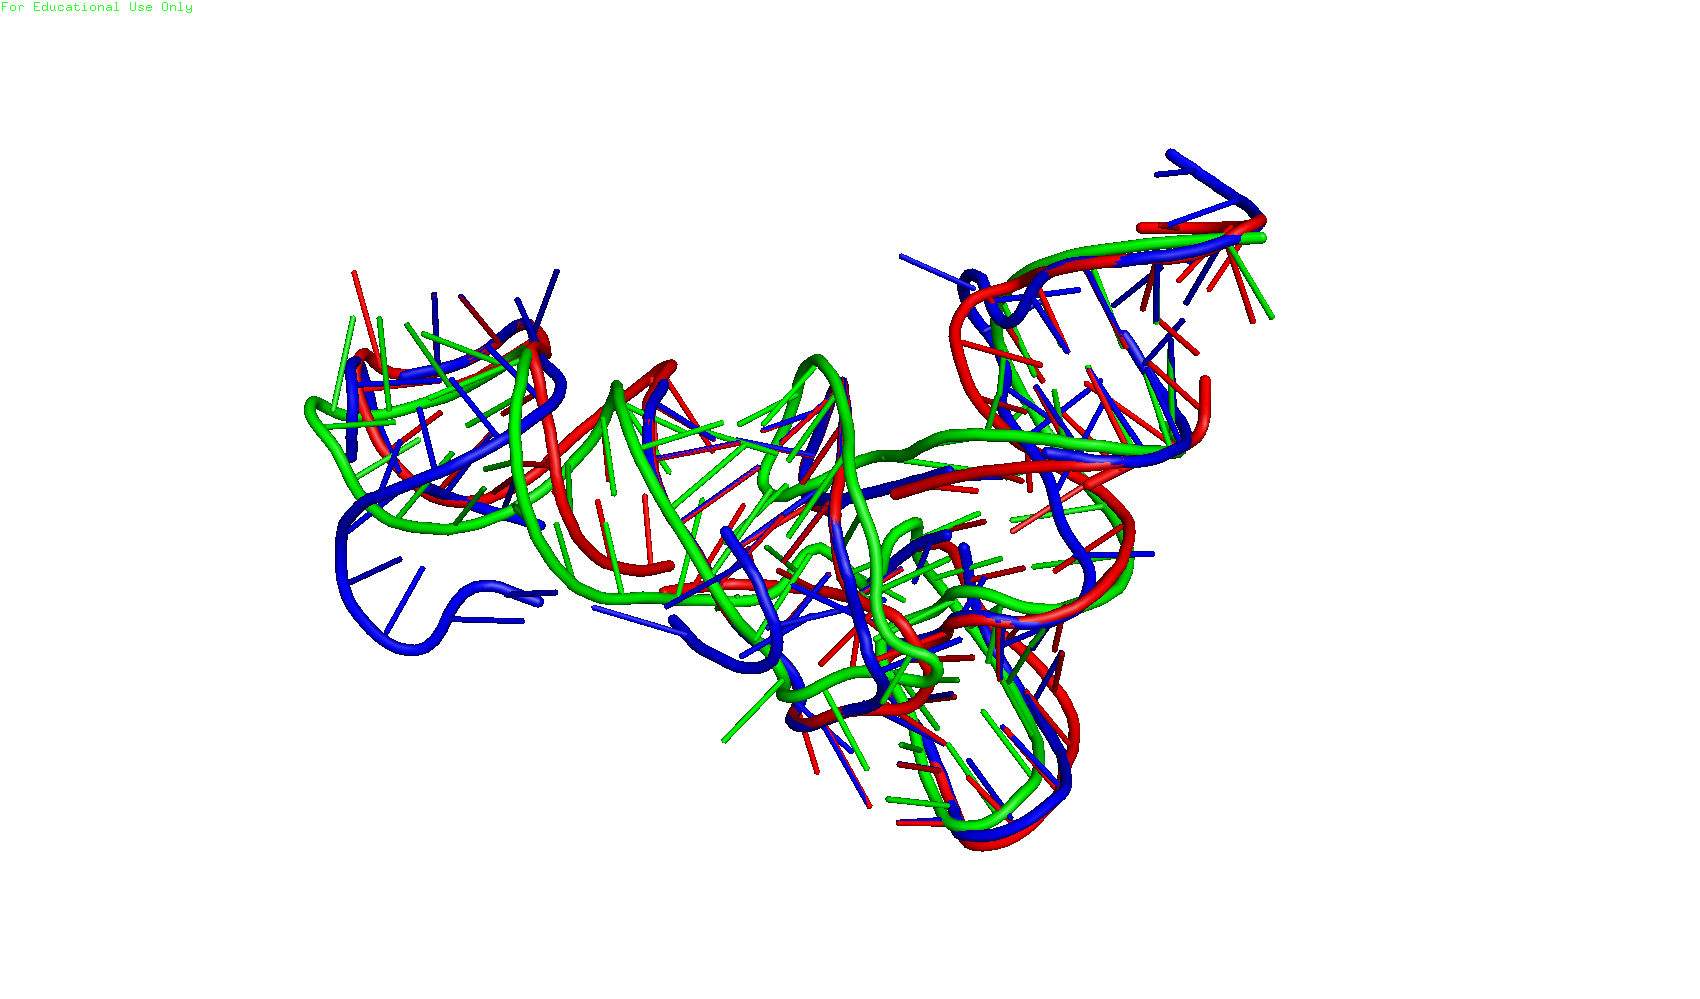
\includegraphics[width=\textwidth]{../img/loss}
\caption{Príklad zhoršenia, v predikcií štruktúry 3L0U\_A pri použití template štruktúry 1FCW\_A spôsobeného použitím viacerých template štruktúr. Zelenou farbou je znázornená experimentálne získana štruktúra, modrou predikcia používajúca viacero template štruktúr (RMSD = 10,764Å) a červenou štruktúra napredikovaná algoritmom z kapitoly 5 (RMSD = 4,58Å). }
\label{obr06.02}
\end{figure}

\begin{figure}%[p]\centering
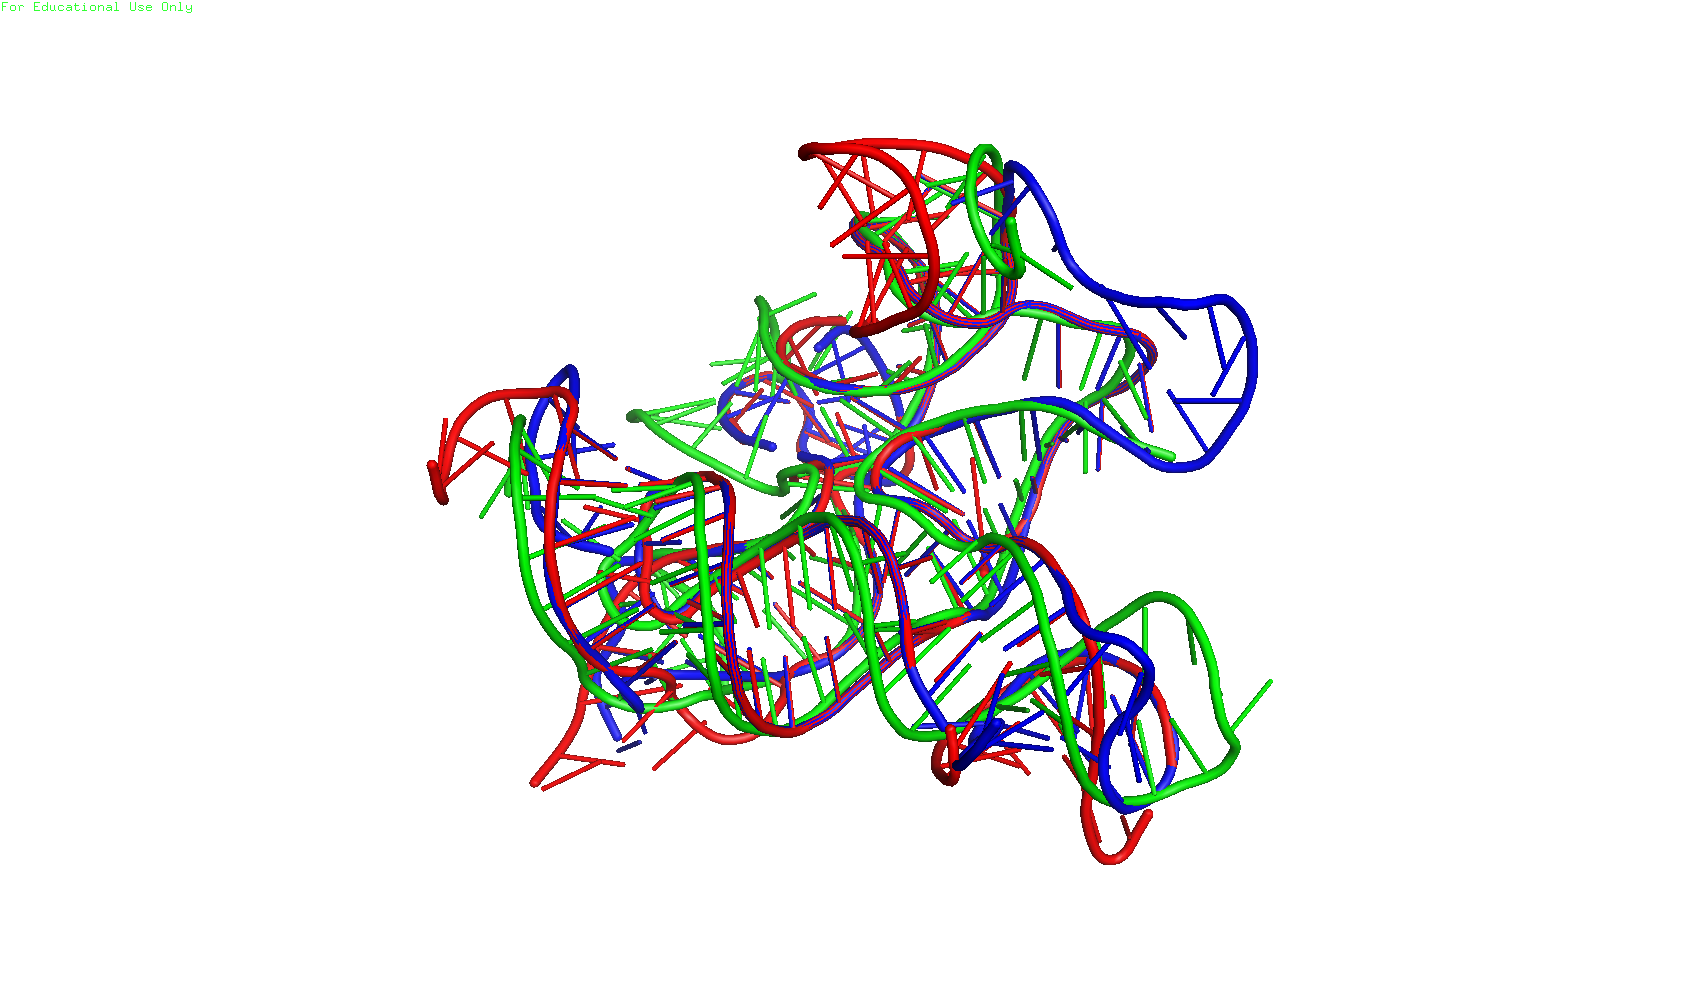
\includegraphics[width=\textwidth]{../img/success}
\caption{Príklad zlepšenia, v predikcií štruktúry 4QLN\_A pri použití template štruktúry 4QK9\_A vďaka použitiu viacerých template štruktúr. Zelenou farbou je znázornená experimentálne získana štruktúra, modrou predikcia používajúca viacero template štruktúr (RMSD = 6,081Å) a červenou štruktúra napredikovaná algoritmom z kapitoly 5 (RMSD = 8,157Å). }
\label{obr06.01}
\end{figure}
